\documentclass[10pt,a4paper]{article}
% \documentclass[a4paper,
% 10pt,
% DIV 10]{scrartcl}

\usepackage[utf8x]{inputenc}
\usepackage[english]{babel}
\usepackage{amssymb}
\usepackage{amsmath}
\usepackage{amsmath}
\usepackage{url}
\usepackage{graphicx}
\usepackage{watermark}
\usepackage{xspace}
\usepackage{paralist}
\usepackage{xargs}
\usepackage{research}

\addtolength{\textheight}{-2cm}
\addtolength{\textwidth}{2cm}
\addtolength{\textheight}{4cm}
\addtolength{\oddsidemargin}{-12mm}

\newcommand*{\atlas}{\textsf{ATLAS}}
\newcommand*{\atlasII}{\textsf{atlas-2}}

\pagestyle{empty}

\begin{document}
\watermark{\put(-95,-760){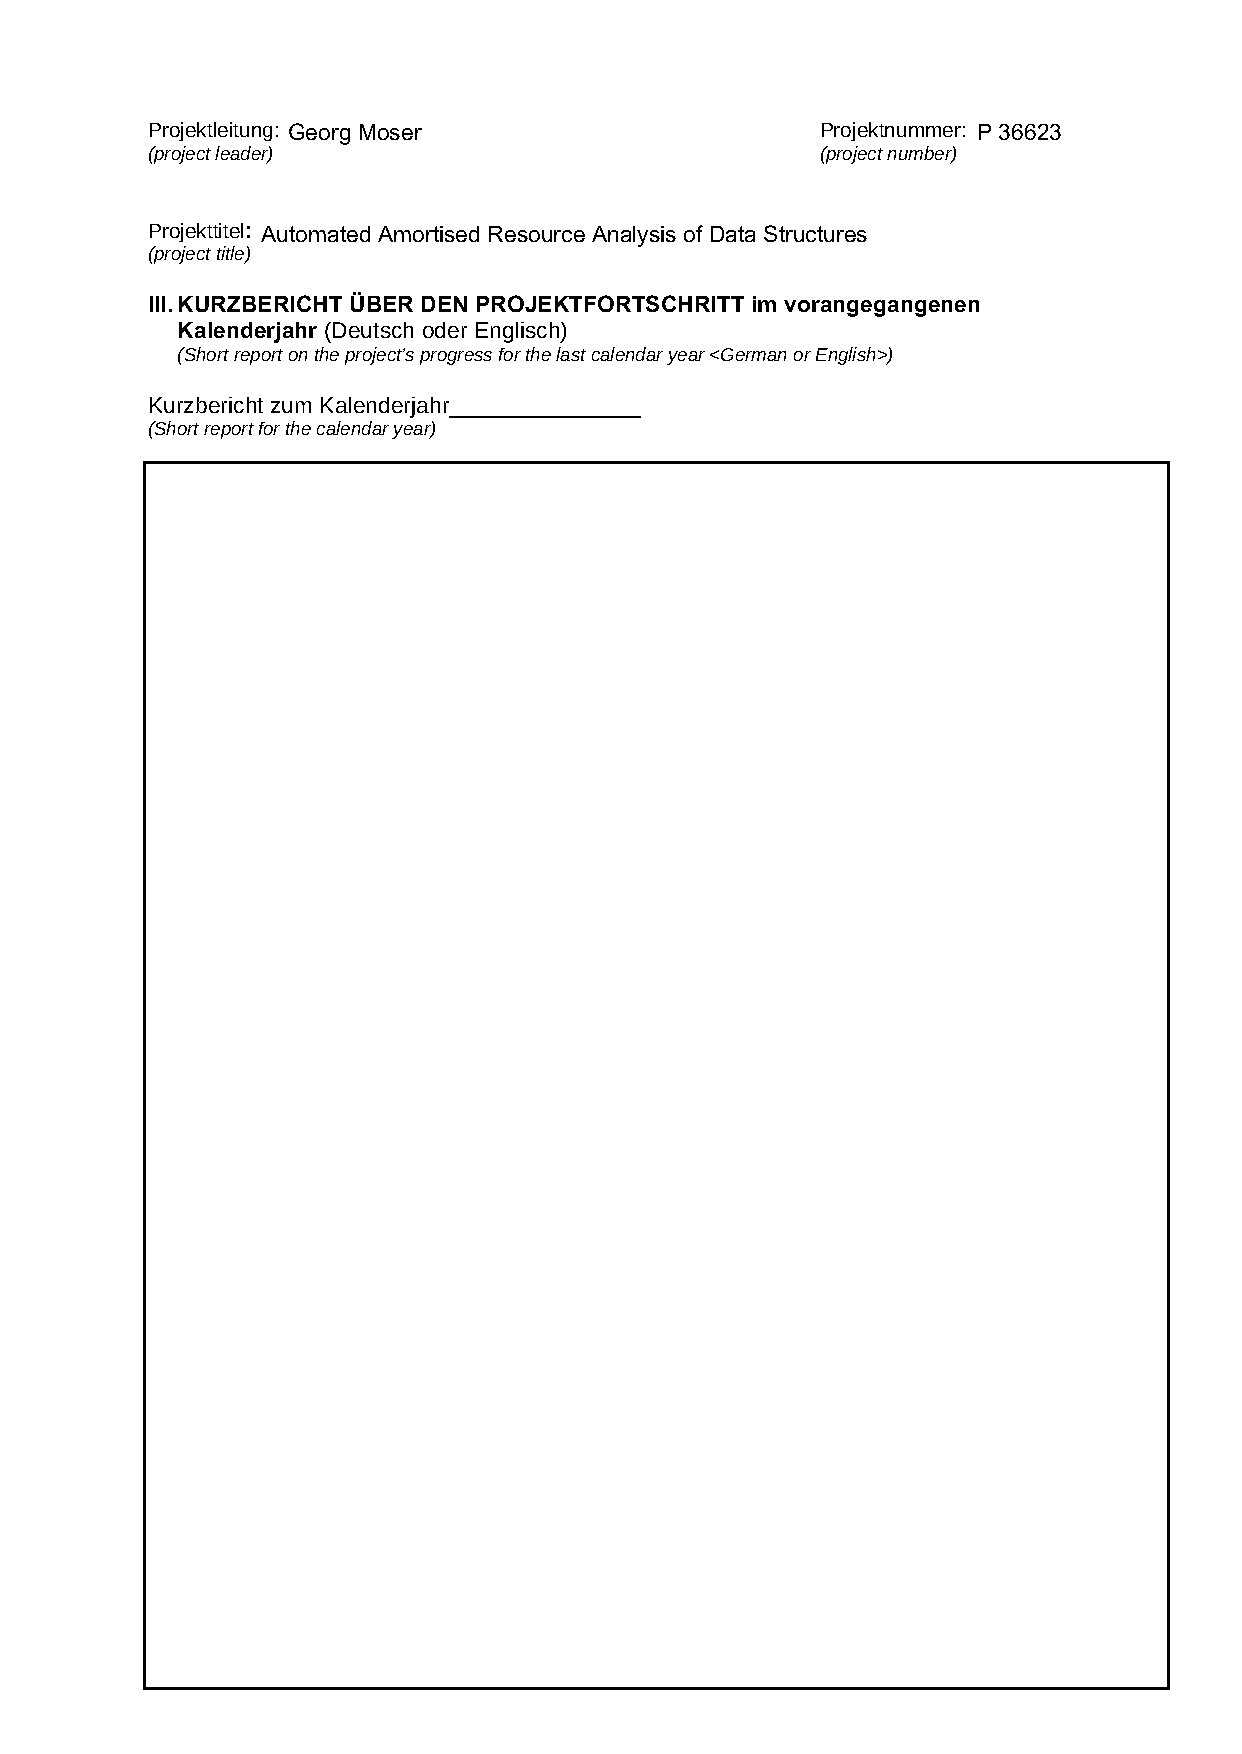
\includegraphics{template.pdf}}}

\vspace*{23mm}
\noindent\hspace{35ex}
2025

\vspace*{10mm}

\begin{center}
\large \normalsize Progress Report AUTOSARD 
\end{center}

After the project's initial phase resulting, among other, in two master thesis on formalisation
of amortised cost analyis of common data structures~\cite{Geser:2024,Hochrainer:2024}, we have
one the one hand continued our work on the formalisation of data structures, but also worked mainly
towards Work Package~1 and~3.

With respect to the formalisation of data structures, we have been intensively working
on the formalisation of \emph{zip trees}, a probabilistic data structure recently developed
by Robert Tarjan, Caleb Levy and Stephen Timmel. Zip trees are isomorphic copies to
\emph{skip lists} introduced in 1990 by William Pugh.
%
In related work, we have provided a formalisation of skip lists based on so-called \emph{weakest-preconditions transformers}~\cite{AvanziniBGMV24}. Partly employing these ideas, but suitably adapted
to the---in our opinion---more elegant zip trees, we have been working on
a formalisation of the expected cost analysis of this data structure in Liquid Haskell, an interactive theorem prover, build on top of the functional
language \Haskell.

Further, we have investigated extensions of our ealier work during the pilot project~\cite{LMZ:2021,LMZ:2022} within Armin Walch's master thesis. Here we have obtained a generalisation of the type system
underlying our prototype~\atlas. This theoretical investigations lead to the (fully) automated amortised
cost analyis of novel algorithms and formed the basis of a complete re-implementation of the prototype. 
In AUTOSARD, we target an automated analysis of the most common data structures with good, ie. sublinear, complexity, such as balanced trees, Fibonacci heaps, randomised search trees, skip lists, skew heaps, Union-find, etc. Our goals are the verification of textbook data structures, the confirmation and improvement (on coefficients) of previously reported complexity bounds, as well as the automated analysis of realistic data structure implementations.

In our initial phase we have started the study and formalisation of sophisticated data structures, like
%
\begin{inparaenum}[(i)]
\item \emph{binomial heaps};
\item \emph{Fibonacci heaps};
\item \emph{rank-balanced trees};
\item \emph{zip trees},
\end{inparaenum}
%
putting in particular emphasis on the correctness and completeness of existing compexity analyses of routine functions
like inseration, deletion, etc. Here we are foremostly interested in amortised complexity analysis that exist for all mentioned
data structures.

With respect to binomial and Fibonacci heaps, as well as rank-balanced trees our efforts resulted in (almost) completed master theses by
Hochrainer~\cite{Hochrainer:2024} and Geser~\cite{Geser:2024}, respectively. In these theses, standard data structure operations in
the corresponding data structures have been formalised in Liquid Haskell, an interactive theorem prover, build on top of the functional
language \Haskell. These gives us complete understanding of the intracties of the various complexity analysis, providing the necessary
ground work for later full automation. Similarly, we have studied zip trees in detail.

We plan a joint publication presenting the results of Geser and Hochrainer. Further, we are working on a journal version for pilot
studies~\cite{LMZ:2021,LMZ:2022} of AUTOSARD, providing a streamlined account of our work on \atlas.
%
For further publication within the project, see~\cite{AvanziniMS23,ParsertP24}.

\bibliographystyle{plain}
\selectlanguage{english}
\small
\bibliography{references}

\end{document}
